\documentclass[a4paper,10pt]{article}
\usepackage[utf8x]{inputenc}
\usepackage[slovene]{babel}
\usepackage{amsmath}
\usepackage{amsfonts}
\usepackage{relsize}
\usepackage[smaller]{acronym}
\usepackage{graphicx}
\usepackage{subfigure}
\usepackage{cite}
\usepackage{url}
\usepackage{hyperref}

\renewcommand{\theta}{\vartheta}
\renewcommand{\phi}{\varphi}

\newcommand{\dd}{\,\mathrm{d}}

\title{Fourierova analiza}
\author{Miha \v Can\v cula}

\begin{document}
  \maketitle

\begin{figure}[h]
  \centering
  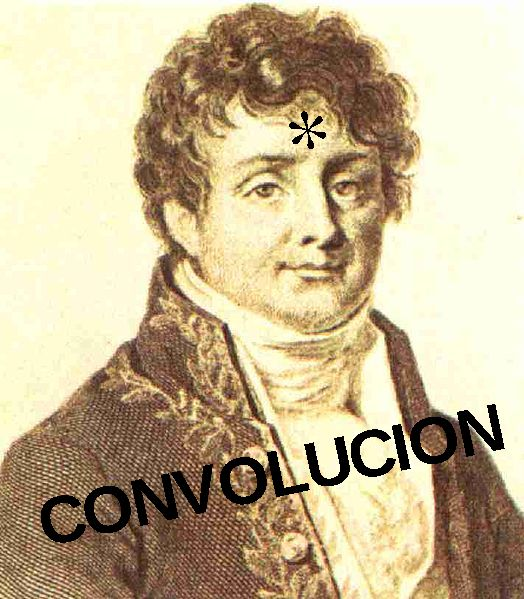
\includegraphics[width=.5\textwidth]{Convolucion}
  \caption{Znani francoski konvolucionar Jean Baptiste Joseph Fourier}
\end{figure}

\section{Konvolucija}

Linearno padajo"co funkcijo $f(x) = 1-x$ sem izvrednostil v $N$ diskretnih to"ckah, nato pa numeri"cno ra"cunal konvolucijo te funkcije samo s sabo. Ta ra"cun sem ponovil pri razli"cnih vrednostih $N$ in ga vsakih napravil na dva na"cina: enkrat po definiciji konvolucije, dru"gi"c pa z uporabo Fourierove transformacije. Za vse ra"cune sem uporabil program \texttt{GNU Octave}. 




\section{Dekonvolucija signala}

Tokrat je bila naloga obratna, poiskati izviren signal ob poznavanju izhodnega signala in prehodne funkcije. Prehodna funkcija $G(t)$ pa je imela en neznani parameter $\beta$, ki sem ga dolocil tako, da je bil izraz

\begin{align}
  \sum_{i=1}^{N-1} \left| s_i - s_{i-1}\right|^2
\end{align}

"cim manj"si. Izka"ze se, da je to pri vrednosti $\beta = 34.852$, vhodni signal pa je tedaj tak kot na sliki~\ref{fig:dekon-signal}. 

\begin{figure}[h]
  \input{g_decon_signal}
\caption{Vhodni in izhodni signal pri $\beta = 34.852$}
\label{fig:dekon-signal}
\end{figure}

\end{document}
